\documentclass[]{article}
\usepackage{amsmath, amsfonts, amssymb, amsthm}
\usepackage{cancel}
\usepackage[output-complex-root=j]{siunitx}
\usepackage[american]{circuitikz}
\usepackage{pgfplots}
\usepackage{bm}
\usepackage{fullpage}
\usepackage{graphicx}
\usepackage{pdfpages}

\renewcommand{\thesection}{\arabic{section}}
\renewcommand{\thesubsection}{\thesection.\alph{subsection}}
\renewcommand{\thesubsubsection}{\thesubsection.\roman{subsubsection}}

\newtheorem{genthm}{Theorem}

\newcommand{\unit}[1]{\bm{\hat{#1}}}
\newcommand{\iprod}[2]{\left\langle #1, #2 \right\rangle}
\newcommand{\tpose}[1]{\left[#1\right]^{\! \top} \!\!}
\newcommand{\diff}[1]{\frac{d}{d #1}}

\title{EECS 16B HW03}
\author{Bryan Ngo}
\date{2020-02-18}

\begin{document}

\maketitle

\section{Complex Numbers}

\subsection{Length of \(z\)}

\begin{equation}
	|z| = \sqrt{x^2 + y^2}
\end{equation}

\subsection{Polar Representation}

\begin{align}
	\Re(z) = x &= r \cos(\theta) \\
	\Im(z) = y &= r \sin(\theta)
\end{align}

\subsection{Euler's Formula}

\begin{align}
	z = x + jy = r \cos(\theta) + jr \sin(\theta) = r(\cos(\theta) + j \sin(\theta)) = re^{j\theta}
\end{align}

\subsection{Unit Complex Circle}

\begin{center}
\begin{tikzpicture}
	\begin{axis}[
		xlabel = {\(\Re\)},
		ylabel = {\(\Im\)},
		xmin = -2, xmax = 2,
		ymin = -2, ymax = 2,
		xtick = {-2,...,2},	ytick = {-2,..., 2},
		yticklabel = {\(\pgfmathprintnumber{\tick}j\)},
		axis lines = middle,
		grid = major,
		axis equal image
	]
	\draw(axis cs:0,0) circle[radius=100];
	\end{axis}
\end{tikzpicture}
\end{center}
\(z\) intersects the real axis at \(z = \pm 1\).
\(z\) intersects the imaginary axis at \(z = \pm j\).

\subsection{}

\begin{proof}
\begin{align}
	z &= re^{j \theta} \\
	re^{-j \theta} &= r \cos(-\theta) + j r \sin(-\theta) \\
	&= r \cos(\theta) - j r \sin(\theta) \\
	&= x - jy = \bar{z}
\end{align}
\end{proof}

\subsection{}

\begin{proof}
\begin{align}
	z \bar{z} &= (x + jy)(x - jy) && \text{definition of conjugate multiplication} \\
	&= x^2 - (jy)^2 && \text{difference of squares} \\
	&= x^2 + y^2 = r^2 && \text{definition of } j
\end{align}
\end{proof}

\section{RLC Responses: Initial Part}

\begin{center}
\begin{circuitikz}\draw
	(0, 0) to[short] (0, 2) to[C=\(C\), v=\(V_C\), i=\(I_L\)] (2, 2) to[R=\(R\), v=\(V_R\)] (4, 2) to[L=\(L\), v=\(V_L\)] (6, 2) to[short] (6, 0) to[short] (0, 0)
;\end{circuitikz}
\end{center}

\subsection{}

Using KVL,
\begin{align}
	V_C + V_R + L \diff{t} I_L &= 0 \\
	C \diff{t} V_C &= I_L
\end{align}
Using simple algebra, we can rearrange to
\begin{align}
	\diff{t} I_L &= -\frac{1}{L} (R I_L + V_C)\\
	\diff{t} V_C &= \frac{1}{C} I_L
\end{align}

\subsection{}

\begin{equation}
	\diff{t}\begin{bmatrix}
	x_1(t) \\
	x_2(t)
	\end{bmatrix} =
	\begin{bmatrix}
	-\frac{R}{L} & -\frac{1}{L} \\
	\frac{1}{C} & 0
	\end{bmatrix}
	\begin{bmatrix}
	x_1(t) \\
	x_2(t)
	\end{bmatrix}
\end{equation}

\subsection{}

\begin{align}
	\begin{vmatrix}
	-\frac{R}{L} - \lambda & -\frac{1}{L} \\
	\frac{1}{C} & -\lambda
	\end{vmatrix} &= \lambda^2 + \frac{R}{L} \lambda + \frac{1}{LC} = 0 \\
	\lambda &= -\frac{R}{2L} \pm \sqrt{\frac{R^2}{4L^2} - \frac{1}{LC}}
\end{align}

\subsection{}

\begin{equation}
	\lambda \in \mathbb{R} \iff \frac{R^2}{4L^2} - \frac{1}{LC} \geqslant 0
\end{equation}

\subsection{}

\begin{equation}
	\lambda \in \{jk | k \in \mathbb{R}, j^2 = -1\} \iff R = 0 \wedge \frac{1}{LC} \geqslant 0
\end{equation}

\subsection{}

Finding the eigenvectors,
\begin{align}
	\begin{bmatrix}
	-\frac{R}{2L} - \sqrt{\frac{R^2}{4L^2} - \frac{1}{LC}} & -\frac{1}{L} \\
	\frac{1}{C} & \frac{R}{2L} - \sqrt{\frac{R^2}{4L^2} - \frac{1}{LC}}
	\end{bmatrix}
	\begin{bmatrix}
	1 \\
	y
	\end{bmatrix}
	&=
	\left(-\frac{R}{2L} + \sqrt{\frac{R^2}{4L^2} - \frac{1}{LC}}\right) \begin{bmatrix}
	1 \\
	y
	\end{bmatrix} \\
	\Rightarrow y_1 &= -2L \sqrt{\frac{R^2}{4L^2} - \frac{1}{LC}} \\
	\bm{v}_1 &= \begin{bmatrix}
	1 \\
	-2L \sqrt{\frac{R^2}{4L^2} - \frac{1}{LC}}
	\end{bmatrix} \\
	\Rightarrow y_2 &= 2L \sqrt{\frac{R^2}{4L^2} - \frac{1}{LC}} \\
	\bm{v_2} &= \begin{bmatrix}
	1 \\
	2L \sqrt{\frac{R^2}{4L^2} - \frac{1}{LC}}
	\end{bmatrix}
\end{align}

\subsection{}

\begin{align}
	\diff{t} \bm{z}(t) &= \begin{bmatrix}
		\lambda_1 & 0 \\
		0 & \lambda_2 
	\end{bmatrix} \bm{z}(t)
\end{align}

\section{RLC Responses: Overdamped Case}

\begin{center}
\begin{circuitikz}\draw
	(0, 0) to[short] (0, 2) to[C=\SI{10}{\nano\farad}, v=\(V_C\), i=\(I_L\)] (2, 2) to[R=\SI{1}{\kilo\ohm}, v=\(V_R\)] (4, 2) to[L=\SI{25}{\micro\henry}, v=\(V_L\)] (6, 2) to[short] (6, 0) to[short] (0, 0)
;\end{circuitikz}
\end{center}

\subsection{}

\begin{align}
	\bm{V} &\approx \begin{bmatrix}
	1 & 1 \\
	-995 & 995
	\end{bmatrix} \\
	\bm{z}(0) &= \bm{V}^{-1} \begin{bmatrix}
	\SI{0}{\ampere} \\
	\SI{1}{\volt}
	\end{bmatrix} \approx
	\begin{bmatrix}
	\num{-502e-6} \\
	\num{502e-6}
	\end{bmatrix}
\end{align}

\subsection{}

\begin{align}
	\lambda_1 &\approx \SI{-100}{\per\kilo\second} \\
	\lambda_2 &\approx \SI{-40}{\per\mega\second} \\
	\bm{z}(t) &= \begin{bmatrix}
	e^{\lambda_1 t} \\
	e^{\lambda_2 t}
	\end{bmatrix} \\
	\bm{x}(t) &= \bm{V} \bm{z}(t) \approx
	\begin{bmatrix}
	1 & 1 \\
	-995 & 995
	\end{bmatrix}
	\begin{bmatrix}
	e^{\lambda_1 t} \\
	e^{\lambda_2 t}
	\end{bmatrix} =
	\begin{bmatrix}
	e^{\lambda_1 t} + e^{\lambda_2 t} \\
	-995 e^{\lambda_1 t} + 995 e^{\lambda_2 t}
	\end{bmatrix}
\end{align}

\subsection{}

\begin{center}
	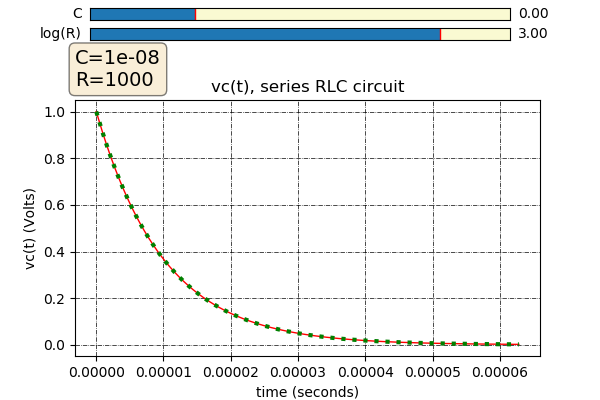
\includegraphics[width=0.7\linewidth]{overdamped}
\end{center}

\begin{center}
	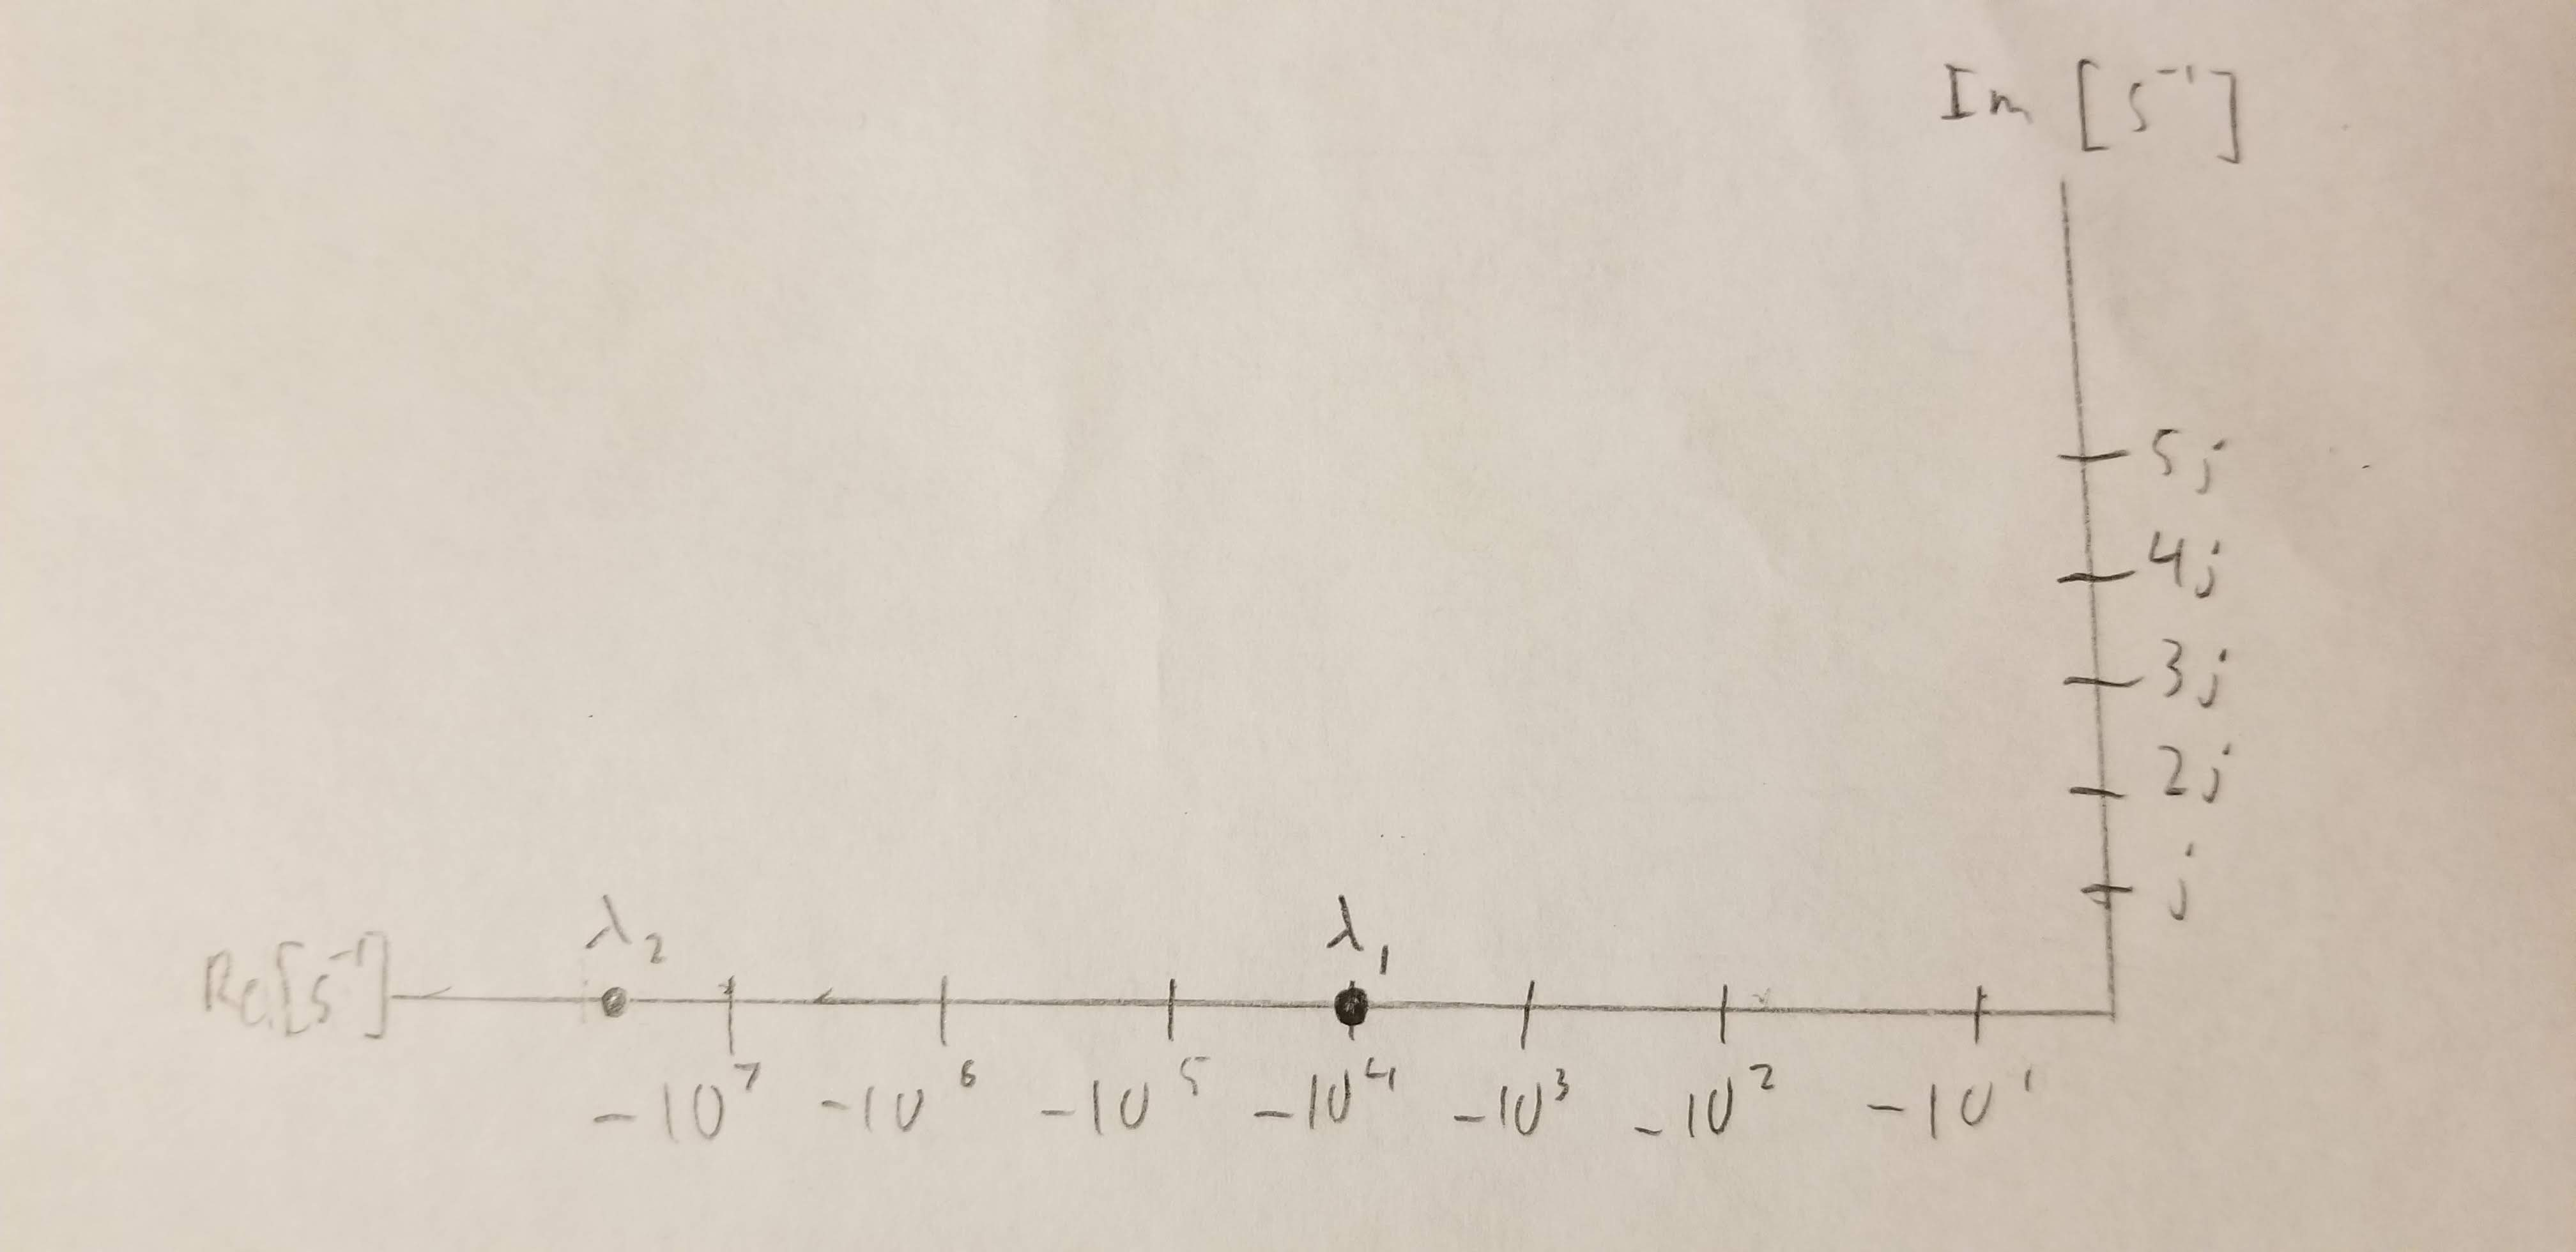
\includegraphics[width=0.7\linewidth]{20200218_233111}
\end{center}
The graph seems to be a plain exponential curve, due to the heavy damping of the resistor.

\section{RLC Responses: Undamped Case}

\begin{center}
\begin{circuitikz}\draw
	(0, 0) to[short] (0, 2) to[C=\SI{10}{\nano\farad}, v=\(V_C\), i=\(I_L\)] (2, 2) to[R=\SI{0}{\ohm}, v=\(V_R\)] (4, 2) to[L=\SI{25}{\micro\henry}, v=\(V_L\)] (6, 2) to[short] (6, 0) to[short] (0, 0)
;\end{circuitikz}
\end{center}

\subsection{}

\begin{align}
	\bm{V} &\approx \begin{bmatrix}
	1 & 1 \\
	-100j & 100j
	\end{bmatrix} \\
	\bm{z}(0) &= \bm{V}^{-1} \begin{bmatrix}
	\SI{0}{\ampere} \\
	\SI{1}{\volt}
	\end{bmatrix} \approx
	\frac{1}{200}\begin{bmatrix}
	-1 \\
	1
	\end{bmatrix}
\end{align}

\subsection{}

\begin{align}
	\lambda_1 &= \SI{2j}{\per\mega\second} \\
	\lambda_2 &= \SI{-2j}{\per\mega\second} \\
	\bm{z}(t) &= \begin{bmatrix}
	e^{\lambda_1 t} \\
	e^{\lambda_2 t}
	\end{bmatrix} \\
	\bm{x}(t) &= \bm{V} \bm{z}(t) =
	\begin{bmatrix}
	1 & 1 \\
	-100j & 100j
	\end{bmatrix}
	\begin{bmatrix}
	e^{\lambda_1 t} \\
	e^{\lambda_2 t}
	\end{bmatrix} =
	\begin{bmatrix}
	e^{\lambda_1 t} + e^{\lambda_2 t} \\
	-100j e^{\lambda_1 t} + 100j e^{\lambda_2 t}
	\end{bmatrix}
\end{align}

\subsection{}

\begin{center}
	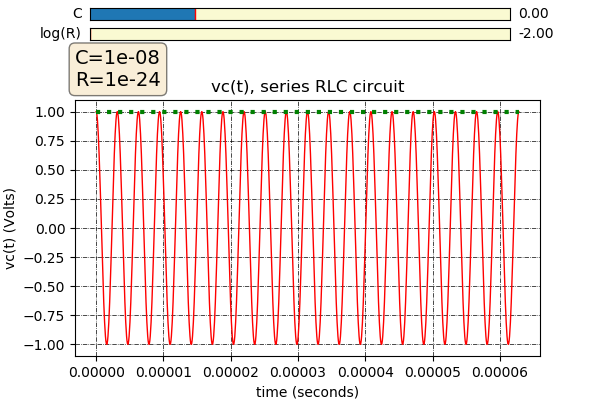
\includegraphics[width=0.7\linewidth]{undamped}
\end{center}

\begin{center}
\begin{tikzpicture}
	\begin{axis}[
		xlabel = {\(\Re\)},
		ylabel = {\(\Im [\si{\per\mega\second}]\)},
		xmin = -2, xmax = 2,
		ymin = -3, ymax = 3,
		xtick = {-2,...,2},	ytick = {-2,..., 2},
		yticklabel = {\(\pgfmathprintnumber{\tick}j\)},
		axis lines = middle,
		grid = major,
	]
		\addplot [only marks, color=blue] coordinates {
			(0, -2) (0, 2)
		};
	\end{axis}
\end{tikzpicture}
\end{center}
The case here shows that the circuit is \emph{not} transient.

\section{RLC Responses: Underdamped Case}

\begin{center}
\begin{circuitikz}\draw
	(0, 0) to[short] (0, 2) to[C=\SI{10}{\nano\farad}, v=\(V_C\), i=\(I_L\)] (2, 2) to[R=\SI{1}{\ohm}, v=\(V_R\)] (4, 2) to[L=\SI{25}{\micro\henry}, v=\(V_L\)] (6, 2) to[short] (6, 0) to[short] (0, 0)
;\end{circuitikz}
\end{center}

\subsection{}

\begin{align}
	\bm{V} &\approx \begin{bmatrix}
	1 & 1 \\
	-100j & 100j
	\end{bmatrix} \\
	\bm{z}(0) &= \bm{V}^{-1} \begin{bmatrix}
	\SI{0}{\ampere} \\
	\SI{1}{\volt}
	\end{bmatrix} \approx
	\frac{1}{200}\begin{bmatrix}
	-1 \\
	1
	\end{bmatrix}
\end{align}

\subsection{}

\begin{align}
	\lambda_1 &= \SI{-20+2000j}{\per\kilo\second} \\
	\lambda_2 &= \SI{-20-2000j}{\per\kilo\second} \\
	\bm{z}(t) &= \begin{bmatrix}
	e^{\lambda_1 t} \\
	e^{\lambda_2 t}
	\end{bmatrix} \\
	\bm{x}(t) &= \bm{V} \bm{z}(t) =
	\begin{bmatrix}
	1 & 1 \\
	-100j & 100j
	\end{bmatrix}
	\begin{bmatrix}
	e^{\lambda_1 t} \\
	e^{\lambda_2 t}
	\end{bmatrix} =
	\begin{bmatrix}
	e^{\lambda_1 t} + e^{\lambda_2 t} \\
	-100j e^{\lambda_1 t} + 100j e^{\lambda_2 t}
	\end{bmatrix}
\end{align}

\subsection{}

\begin{center}
	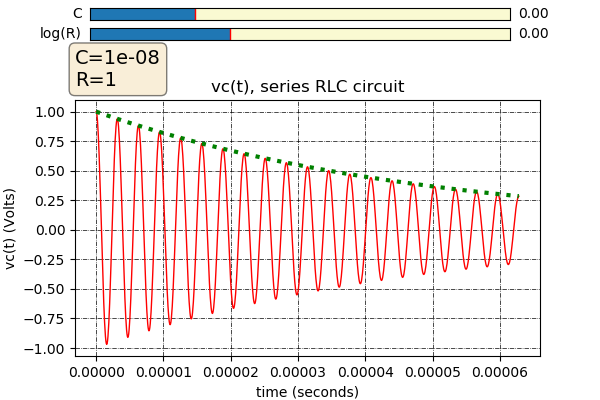
\includegraphics[width=0.7\linewidth]{underdamped}
\end{center}

\begin{center}
	\begin{tikzpicture}
	\begin{axis}[
	xlabel = {\(\Re [\si{\per\mega\second}]\)},
	ylabel = {\(\Im [\si{\per\mega\second}]\)},
	xmin = -2, xmax = 2,
	ymin = -3, ymax = 3,
	xtick = {-2,...,2},	ytick = {-2,..., 2},
	yticklabel = {\(\pgfmathprintnumber{\tick}j\)},
	axis lines = middle,
	grid = major,
	]
	\addplot [only marks, color=blue] coordinates {
		(-0.2, -2) (-0.2, 2)
	};
	\end{axis}
	\end{tikzpicture}
\end{center}
The graph appears to exhibit transient behavior, due to the asymptotic decline.

\subsection{}

Even though \(\lambda_1, \lambda_2 \in \mathbb{C}\), it can be shown that the differential equation is nothing more than a linear combination of sine and cosine waves multiplied by an exponential function, due to the fact that
\begin{align}
	\sin(t) &= \frac{e^{jt} - e^{-jt}}{2j} \\
	\cos(t) &= \frac{e^{jt} + e^{-jt}}{2}
\end{align}

\section{RLC Responses: Critically Damped}

\subsection{}

There will only be one eigenvalue of \(A\) when \(\frac{R^2}{4L^2} = \frac{1}{LC} \Rightarrow R = 2\sqrt{\frac{L}{C}}\).

\subsection{}

\begin{align}
	\begin{vmatrix}
	-\frac{2}{L} \sqrt{\frac{L}{C}} - \lambda & -\frac{1}{L} \\
	\frac{1}{C} & -\lambda
	\end{vmatrix} &= \lambda^2 + \frac{2}{L} \sqrt{\frac{L}{C}} \lambda + \frac{1}{LC} = 0 \\
	\lambda &= -2 \frac{1}{\sqrt{LC}}
\end{align}

\begin{align}
	\begin{bmatrix}
	0 & \frac{-1}{L} \\
	\frac{1}{C} & \frac{2}{\sqrt{LC}}
	\end{bmatrix}
	\begin{bmatrix}
	1 \\
	y
	\end{bmatrix}
	&=
	-\frac{2}{\sqrt{LC}} \begin{bmatrix}
	1 \\
	y
	\end{bmatrix} \\
	y &= \frac{2L}{\sqrt{LC}}, -\frac{\sqrt{LC}}{4C}
\end{align}
Thus, we are able to find 2 eigenvectors for the eigenspace.

\subsection{}

\begin{center}
	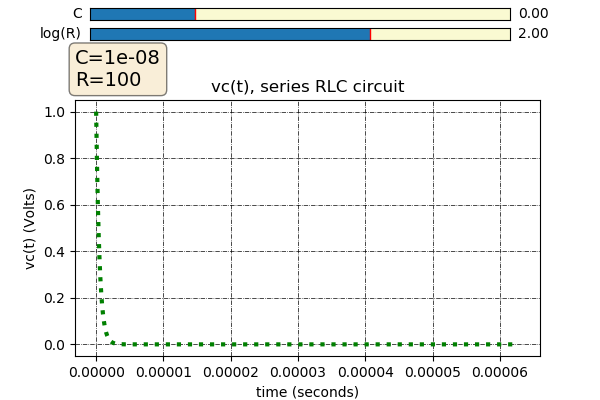
\includegraphics[width=0.7\linewidth]{critdamped}
\end{center}

\begin{center}
\begin{tikzpicture}
	\begin{axis}[
		xlabel = {\(\Re [\si{\per\mega\second}]\)},
		ylabel = {\(\Im [\si{\per\mega\second}]\)},
		xmin = -3, xmax = 2,
		ymin = -3, ymax = 3,
		xtick = {-2,...,2},	ytick = {-2,..., 2},
		yticklabel = {\(\pgfmathprintnumber{\tick}j\)},
		axis lines = middle,
		grid = major,
	]
		\addplot [only marks, color=blue] coordinates {
			(-2, 0)
		};
	\end{axis}
\end{tikzpicture}
\end{center}
The graph seems to decay faster than at any other eigenvalue.
If \(R\) is shifted up, then it becomes overdamped and the curve shallows.
If \(R\) is shifted down, then it becomes underdamped and begins to oscillate.

\stepcounter{section}

\section{Homework Process and Study Group}

\begin{enumerate}
	\item I referred to Note 3, Discussion 3B, and my lecture notes.
	\item I worked on this homework by myself.
	\item I did this homework in one sitting.
	\item Around 4.5 hours.
\end{enumerate}

\newpage

%\includepdf[pages=-]{prob*.pdf}

\end{document}
